\documentclass{article}

\usepackage{mathtools, commath}

% Packages for formatting
\usepackage[margin=1in]{geometry}
\usepackage{fancyhdr}
\usepackage{enumerate}
\usepackage{graphicx}
\usepackage{kotex}
\usepackage{amsmath}
\usepackage{amsthm}
\usepackage[table]{xcolor}
\usepackage{amssymb, amsfonts}

% Fonts
%\usepackage[T1]{fontenc}
%\usepackage[utf8]{inputenc}
%\usepackage{newpxtext,newpxmath}
%\usepackage{sectsty}
%\usepackage{helvet}
%\usepackage{avant}
%\renewcommand*\familydefault{\sfdefault}
%\usepackage{textcomp}

%\usepackage[T1]{fontspec}
%\usepackage{newpxtext,newpxmath}
%\setmainfont{TeX Gyre Termes}
%\setsansfont[
%Path = fonts/,
%UprightFont = *Medium.ttf,
%BoldFont    = *Bold.ttf,
%AutoFakeSlant = 0.2
%]{GmarketSansTTF}
\usepackage{fontspec}
\usepackage{unicode-math} % The modern replacement for newpxmath

% Set the main serif text font (Times clone)
\setmainfont{TeX Gyre Termes}

% Set the matching math font
\setmathfont{TeX Gyre Termes Math} 

% Set the sans-serif font using your local .ttf files
\setsansfont[
Path = fonts/,
UprightFont = *Medium.ttf,
BoldFont = *Bold.ttf,
AutoFakeSlant = 0.2
]{GmarketSansTTF}

% Define colors
\definecolor{blue1}{HTML}{0077c2}
\definecolor{blue2}{HTML}{00a5e6}
\definecolor{blue3}{HTML}{b3e0ff}
\definecolor{blue4}{HTML}{00293c}
\definecolor{blue5}{HTML}{e6f7ff}

\definecolor{thmcolor}{RGB}{231, 76, 60}
\definecolor{defcolor}{RGB}{52, 152, 219}
\definecolor{lemcolor}{RGB}{155, 89, 182}
\definecolor{corcolor}{RGB}{46, 204, 113}
\definecolor{procolor}{RGB}{241, 196, 15}

\usepackage{color,soul}
\usepackage{soul}
\newcommand{\mathcolorbox}[2]{\colorbox{#1}{$\displaystyle #2$}}
\usepackage{cancel}
\newcommand\crossout[3][black]{\renewcommand\CancelColor{\color{#1}}\cancelto{#2}{#3}}
\newcommand\ncrossout[2][black]{\renewcommand\CancelColor{\color{#1}}\cancel{#2}}

\usepackage{hyperref}
\usepackage{booktabs}

% Chapter formatting
\definecolor{titleblue}{RGB}{0,53,128}
\usepackage{titlesec}
\titleformat{\section}
{\normalfont\sffamily\Large\bfseries\color{titleblue!100!gray}}{\thesection}{1em}{}
\titleformat{\subsection}
{\normalfont\sffamily\large\bfseries\color{titleblue!50!gray}}{\thesubsection}{1em}{}

%Tcolorbox
\usepackage[most]{tcolorbox}

%Tikzpicture
\usepackage{tikz-cd}
\usetikzlibrary{positioning}
\usetikzlibrary{angles, quotes}
\usetikzlibrary{patterns,patterns.meta}

\usepackage[linesnumbered,ruled]{algorithm2e}
\usepackage{algpseudocode}
\usepackage{setspace}
\SetKwComment{Comment}{/* }{ */}
\SetKwProg{Fn}{Function}{:}{end}
\SetKw{End}{end}
\SetKw{DownTo}{downto}

% Define a new environment for algorithms without line numbers
\newenvironment{algorithm2}[1][]{
	% Save the current state of the algorithm counter
	\newcounter{tempCounter}
	\setcounter{tempCounter}{\value{algocf}}
	% Redefine the algorithm numbering (remove prefix)
	\renewcommand{\thealgocf}{}
	\begin{algorithm}
	}{
	\end{algorithm}
	% Restore the algorithm counter state
	\setcounter{algocf}{\value{tempCounter}}
}

\usepackage{listings}

\lstset{
	basicstyle=\footnotesize\ttfamily,
	breaklines=true,
	frame=single,
	columns=fullflexible,
	captionpos=b,
	postbreak=\mbox{\textcolor{red}{$\hookrightarrow$}\space},
	numbers=none,
	tabsize=4,
	keepspaces=true,
	showspaces=false,
	showstringspaces=false,
	showtabs=false
}

\lstdefinelanguage{SageMath}{
	language=Python,
	morekeywords={
		var, plot, list_plot, matrix, vector, identity_matrix,
		random_matrix, GF, QQ, RR, ZZ, prod, factor, expand,
		show, graphics_array
	},
	sensitive=true,
	morecomment=[l]\#,
	morestring=[b]',
	morestring=[b]"
}

\lstdefinestyle{sagemath}{
	language=SageMath,
	basicstyle=\ttfamily\small,
	keywordstyle=\color{blue},
	commentstyle=\color{green!50!black},
	stringstyle=\color{red!60!black},
	numbers=left,
	numberstyle=\tiny\color{gray},
	stepnumber=1,
	numbersep=8pt,
	frame=single,
	breaklines=true,
	columns=fullflexible,
	keepspaces=true,
	showspaces=false,
	showstringspaces=false,
	showtabs=false
}

% Header and footer formatting
\pagestyle{fancy}
\fancyhead{}
\fancyhf{}
\rhead{\sffamily \large Student ID: F2025014\quad Name: \textbf{지용현}}%\rule{3cm}{0.4pt}}
\lhead{\textcolor{blue2}{\sffamily\large\textbf{[2026-1] 고급정보통신론}}}
% Define footer
\newcommand{\footer}[1]{
\begin{flushright}
	\vspace{2em}
	
\includegraphics[width=3.5cm]{school_logo.jpg} \\
	\vspace{1em}
	\textcolor{blue2}{\sffamily\large\textbf{#1}}
\end{flushright}
}
%\rfoot{\large Department of Information Security, Cryptogrphy and Mathematics, Kookmin Uni.
\includegraphics[height=1.5cm]{school_logo.jpg}}
\fancyfoot{}
\fancyfoot[C]{-\thepage-}

\newcommand{\ie}{\textnormal{i.e.}}
\newcommand{\rsa}{\mathsf{RSA}}
\newcommand{\rsacrt}{\mathsf{RSA}\textendash\mathsf{CRT}}
\newcommand{\inv}[1]{#1^{-1}}

\usepackage{amsthm}
\newtheorem{axiom}{Axiom}[section]
\newtheorem{theorem}{Theorem}
\newtheorem*{theorem*}{Theorem}
\newtheorem{proposition}[theorem]{Proposition}
\newtheorem{corollary}{Corollary}[theorem]
\newtheorem*{corollary*}{Corollary}
\newtheorem{lemma}[theorem]{Lemma}
\newtheorem*{lemma*}{Lemma}

\theoremstyle{definition}
\newtheorem{definition}{Definition}
\newtheorem*{definition*}{Definition}
\newtheorem{remark}{Remark}
\newtheorem{exercise}{Exercise}[section]
\newtheorem*{note}{Note}
\newtheorem*{notation}{Notation}
\newtheorem{example}{Example}
\newtheorem*{observation}{\color{magenta}Obervation}

%New Command
%\newcommand{\set}[1]{\left\{#1\right\}}
\newcommand{\N}{\mathbb{N}}
\newcommand{\Z}{\mathbb{Z}}
\newcommand{\Q}{\mathbb{Q}}
\newcommand{\R}{\mathbb{R}}
\newcommand{\C}{\mathbb{C}}
\newcommand{\F}{\mathbb{F}}
\newcommand{\nbhd}{\mathcal{N}}
\newcommand{\Log}{\operatorname{Log}}
\newcommand{\Arg}{\operatorname{Arg}}
\newcommand{\pv}{\operatorname{P.V.}}
%\newcommand{\F}{\mathbb{F}}
\newcommand{\GL}{\operatorname{GL}}
\newcommand{\rank}{\operatorname{rank}}
\newcommand{\im}{\operatorname{Im}}
\newcommand{\Ker}{\operatorname{Ker}}
\newcommand{\Span}{\operatorname{Span}}
\newcommand{\Prob}{\mathbb{P}}
\newcommand{\cC}{\mathcal{C}}
\newcommand{\Mat}{\operatorname{Mat}}

\newcommand{\of}[1]{\left( #1 \right)} 
%\newcommand{\abs}[1]{\left\lvert #1 \right\rvert}
%\newcommand{\norm}[1]{\left\| #1 \right\|}

\newcommand{\sol}{\textcolor{magenta}{\bf Sol}}
\newcommand{\conjugate}[1]{\overline{#1}}

\newcommand{\res}{\operatorname{res}}
\DeclareMathOperator*{\Res}{\operatorname{Res}}

\renewcommand{\Re}{\operatorname{Re}}
\renewcommand{\Im}{\operatorname{Im}}

\newcommand{\cyclic}[1]{\langle #1 \rangle}
\newcommand{\uniform}{\overset{\$}{\leftarrow}}

\renewcommand{\emph}[1]{\textbf{#1}}

\definecolor{axiomcolor}{HTML}{a88bfa}
\definecolor{defcolor}{RGB}{52, 152, 219}
\definecolor{procolor}{RGB}{241, 196, 15}
\definecolor{thmcolor}{RGB}{231, 76, 60}
\definecolor{lemcolor}{RGB}{155, 89, 182}
\definecolor{corcolor}{RGB}{46, 204, 113}
\definecolor{execolor}{RGB}{90, 128, 127}

\usepackage{blochsphere}
\usepackage{braket}

%------------------------------------------------------------------
% Global parameters for the Bloch sphere and state coordinates
\def\rotationSphere{-110}  % Viewing rotation for the sphere
\def\radiusSphere{4cm}     % Sphere radius
\def\psiLat{45}            % Initial polar angle θ (in degrees)
\def\psiLon{45}            % Initial azimuth φ (in degrees)
% Note: The state is placed as \labelLatLon{psi}{\psiLat}{-\psiLon}.

\begin{document}
\pagenumbering{arabic}
\begin{center}
	\huge\textbf{HW\#1: Counting Invertible Matrices}\\
	\vspace{0.5em}
\end{center}

\begin{notation}
	We denote the space of $m\times m$ matrices over a finite field $\F_q$ by $\mathrm{Mat}_m(\F_q)$ instead of $\F_q^{m\times m}$.
\end{notation}


\begin{tcolorbox}[colback=white, colframe=axiomcolor,title={\textbf{Cardinality of the matrix space \(\mathrm{Mat}_m(\F_q)\)}}]
\begin{proposition}
Let \(m,n\in \mathbb{Z}_{>0}\), and let \(q\) be a prime power. The number of \(m\times n\) matrices over the finite field \(\F_q\) is \[
\bigl|\mathrm{Mat}_m(\F_q)\bigr|=q^{mn}.
\]
In particular, \[
\bigl|\mathrm{Mat}_m(\F_q)\bigr|=q^{m^2}.
\]
\end{proposition}
\end{tcolorbox}

%\begin{proof}
%We write an arbitrary matrix $A\in\mathrm{Mat}_{m\times n}(\F_q)$ in matrix form: \[
%A=
%\begin{pmatrix}
%	a_{11} & a_{12} & \cdots & a_{1n}\\
%	a_{21} & a_{22} & \cdots & a_{2n}\\
%	\vdots & \vdots & \ddots & \vdots\\
%	a_{m1} & a_{m2} & \cdots & a_{mn}
%\end{pmatrix},
%\qquad a_{ij}\in \F_q.
%\]To specify such a matrix, we must choose each entry
%\[
%a_{11},a_{12},\dots,a_{1n},
%a_{21},a_{22},\dots,a_{2n},
%\dots,
%a_{m1},a_{m2},\dots,a_{mn}.
%\]
%There are exactly \(mn\) entries altogether.
%
%Since \(\F_q\) has exactly \(q\) elements, each entry \(a_{ij}\) has \(q\) possible choices. Thus \[
%\begin{array}{cccccc}
%	a_{11} & a_{12} & \cdots & a_{1n} & \cdots & a_{mn}\\
%	q & q & \cdots & q & \cdots & q
%\end{array}
%\]
%By the product rule, the total number of matrices is \[
%\underbrace{q\cdot q\cdot \dots \cdot q}_{mn\text{ factors}}
%=
%q^{mn}.
%\]
%Therefore
%\[
%\bigl|\mathrm{Mat}_{m\times n}(\F_q)\bigr|=q^{mn}.
%\]
%In the case \(n=m\), we get
%\[
%\bigl|\mathrm{Mat}_m(\F_q)\bigr|
%=
%q^{m\cdot m}
%=
%q^{m^2}.
%\]
%\end{proof}

%\newpage

\medskip

\begin{tcolorbox}[colback=white, colframe=defcolor,title={\textbf{General linear group}}]
\begin{definition}
	The \emph{general linear group} over \(\F_q\) is
	\[
	\GL_m(\F_q) := \{A\in \mathrm{Mat}_{m\times m}(\F_q) : A \text{ is invertible}\}.
	\]
\end{definition}
\end{tcolorbox}
\begin{remark}
	$\GL_m(\F_q)=\set{A\in\mathrm{Mat}_{m\times m}(\F_q):\det A\neq 0}=\mathrm{Mat}_{m\times m}(\F_q)\setminus\set{A\in\mathrm{Mat}_{m\times m}(\F_q):\det A = 0}$.
\end{remark}

\begin{remark}
	Let
	\[
	A=
	\begin{pmatrix}
		| & | & & |\\
		\textbf{v}_1 & \textbf{v}_2 & \cdots & \textbf{v}_m\\
		| & | & & |
	\end{pmatrix}
	\in \mathrm{Mat}_{m\times m}(\F_q),
	\]
	where \(\textbf{v}_i\in \F_q^m\) are the columns of \(A\). Then \(A\) is invertible if and only if its columns are linearly independent.
	\begin{center}
		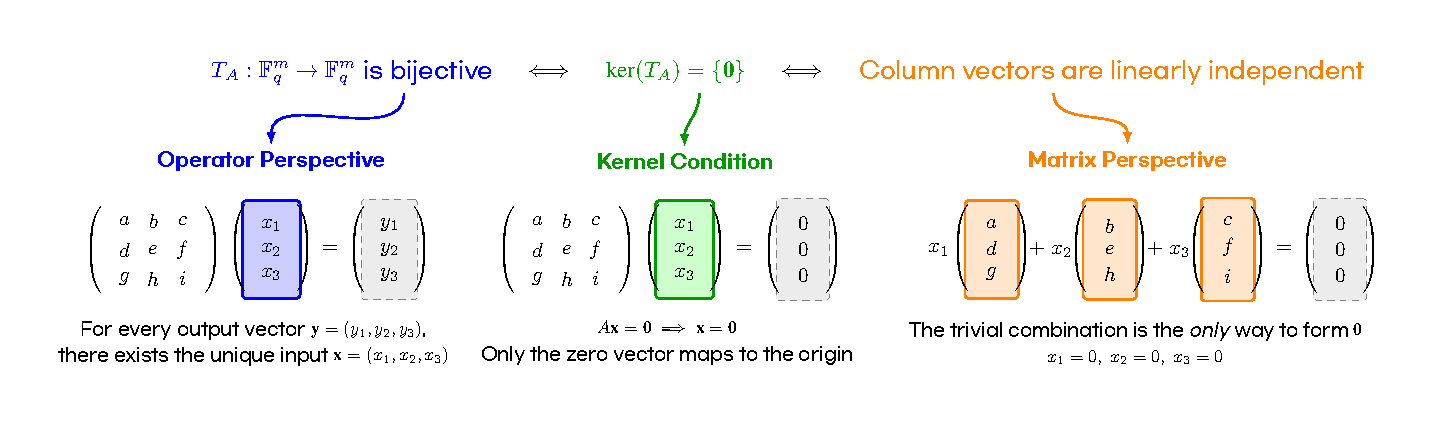
\includegraphics[width=\textwidth]{tikz/HW1-invertible.pdf}
	\end{center}
\end{remark}

%\newpage

\begin{observation}[Computation of \(|GL_1(\F_q)|\)]
\; \begin{center}
\begin{minipage}{.48\textwidth}
A \(1\times 1\) matrix has the form
\[
A=\begin{pmatrix} a \end{pmatrix}=a, \qquad a\in \F_q.
\]
Such a matrix is invertible iff \(a\neq 0\). Therefore \[
GL_1(\F_q)=\left\{a: a\in \F_q^\times\right\},
\]
and hence
\[
|GL_1(\F_q)|=|\F_q^\times|=q-1.
\]
\end{minipage}
\begin{minipage}{.48\textwidth}\centering
	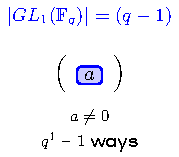
\includegraphics[width=.7\textwidth]{tikz/HW1-card-gl_1.pdf}
\end{minipage}
\end{center}
\end{observation}

\newpage

\begin{observation}[Computation of \(|GL_2(\F_q)|\)]
\; \begin{center}
\begin{minipage}{.49\textwidth}
A \(2\times 2\) matrix has the form
\[
A=\begin{pmatrix}
	a & b\\
	c & d
\end{pmatrix},
\qquad a,b,c,d\in \F_q.
\] Write the columns as
\[
\textbf{v}_1=\begin{pmatrix} a\\ c \end{pmatrix},
\qquad
\textbf{v}_2=\begin{pmatrix} b\\ d \end{pmatrix}.
\]
\end{minipage}
\begin{minipage}{.49\textwidth}\centering
	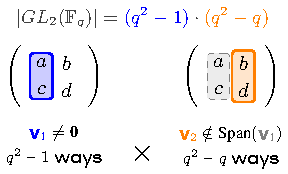
\includegraphics[width=.8\textwidth]{tikz/HW1-card-gl_2.pdf}
\end{minipage}
\end{center}
\begin{enumerate}[(i)]
	\item The vector \(\textbf{v}_1\) can be any nonzero vector in \(\F_q^2\). Hence there are
	$q^2-1$ choices.
	\item Since \(\Span(\textbf{v}_1)=\set{\lambda\textbf{v}_1:\lambda\in\F_q}\) has exactly \(q\) elements, there are
	$q^2-q$ choices for \(\textbf{v}_2\).
\end{enumerate}
	Multiplying these choices, we obtain
	\[
	|GL_2(\F_q)|=(q^2-1)(q^2-q).
	\]
\end{observation}

\medskip

\begin{observation}[Computation of \(|GL_3(\F_q)|\)]
\; \begin{center}
%	\begin{minipage}{.49\textwidth}
%A \(3\times 3\) matrix has the form
%\[
%A=
%\begin{pmatrix}
%	a & b & c\\
%	d & e & f\\
%	g & h & i
%\end{pmatrix},
%\] $a,b,c,d,e,f,g,h,i\in \F_q.$
%Write the columns as
%\[
%\textbf{v}_1=
%\begin{pmatrix}
%	a\\ d\\ g
%\end{pmatrix},
%\qquad
%\textbf{v}_2=
%\begin{pmatrix}
%	b\\ e\\ h
%\end{pmatrix},
%\qquad
%\textbf{v}_3=
%\begin{pmatrix}
%	c\\ f\\ i
%\end{pmatrix}.
%\]
%\end{minipage}
%	\begin{minipage}{.49\textwidth}\centering
%		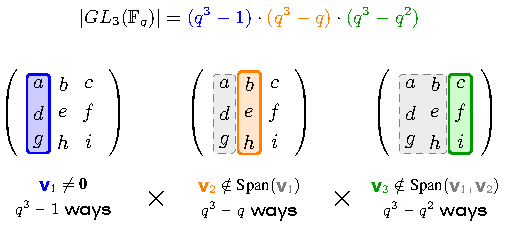
\includegraphics[width=1\textwidth]{tikz/HW1-card-gl_3.pdf}
%	\end{minipage}
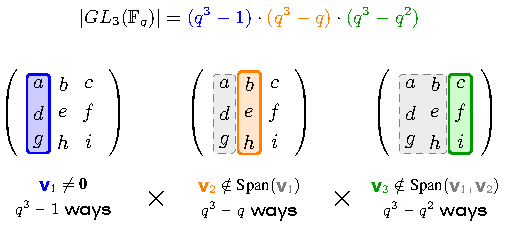
\includegraphics[scale=1.4]{tikz/HW1-card-gl_3.pdf}
\end{center}
%\begin{enumerate}[(i)]
%	\item The vector \(\textbf{v}_1\) can be any nonzero vector in \(\F_q^3\). Hence there are $
%	q^3-1$ choices.
%	\item Since \(\Span(\textbf{v}_1)\) has exactly \(q\) elements, there are $
%	q^3-q$ choices for \(\textbf{v}_2\).
%	\item Since \(\textbf{v}_1\) and \(\textbf{v}_2\) are linearly independent, their span is a \(2\)-dimensional subspace of \(\F_q^3\), so it has exactly \(q^2\) elements. Therefore there are $
%	q^3-q^2$ choices for \(v_3\).
%\end{enumerate}
%Multiplying these choices, we obtain
%\[
%|GL_3(\F_q)|=(q^3-1)(q^3-q)(q^3-q^2).
%\]
\end{observation}

\medskip

\begin{observation}[Computation of \(|GL_4(\F_q)|\)]
	\; \begin{center}
			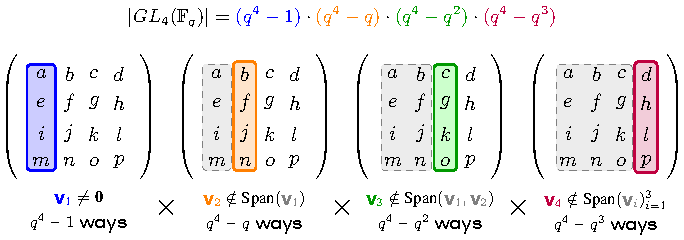
\includegraphics[scale=1.4]{tikz/HW1-card-gl_4.pdf}
		\end{center}
\end{observation}

\newpage
\begin{tcolorbox}[colback=white, colframe=axiomcolor,title={\textbf{Counting invertible matrices over a finite field \(\F_q\)}}]
\begin{theorem}
Let \(m,n\in \mathbb{Z}_{>0}\), and let \(q\) be a prime power.
The number of invertible \(m\times m\) matrices over \(\F_q\) is \[
|\GL_m(\F_q)| = (q^m-1)(q^m-q)(q^m-q^2)\cdots(q^m-q^{m-1}).
\]
Equivalently, \[
|\GL_m(\F_q)| = \prod_{i=0}^{m-1}(q^m-q^i).
\]
%The number of invertible \(m\times m\) matrices over \(\F_q\) is \[
%|\GL_m(\F_q)| = (q^m-1)(q^m-q)(q^m-q^2)\cdots(q^m-q^{m-1})
%= \prod_{i=0}^{m-1}(q^m-q^i).
%\]
\end{theorem}
\end{tcolorbox}

\begin{remark}
\; \begin{center}
	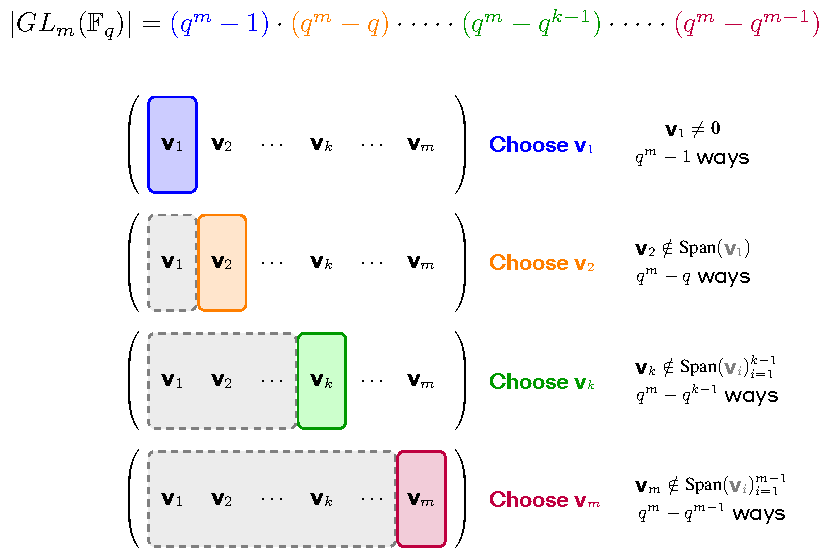
\includegraphics[width=.8\textwidth]{tikz/HW1-card-gl_m.pdf}
\end{center}
\end{remark}

%\begin{proof}
%	We count invertible matrices by choosing their columns.
%	\begin{itemize}
%		\item The first column can be any nonzero vector of \(\F_q^m\), so there are \(q^m-1\) choices.
%		\item The second column must not lie in the span of the first column. Since the span of one nonzero vector has \(q\) elements, there are \(q^m-q\) choices.
%		\item The third column must not lie in the span of the first two columns. If those are independent, their span has \(q^2\) elements, so there are \(q^m-q^2\) choices.
%		\item Continuing this way, the \(k\)-th column must avoid a subspace of size \(q^{k-1}\), so there are \(q^m-q^{k-1}\) choices.
%	\end{itemize}
%	Multiplying all factors gives
%	\[
%	|\GL_m(\F_q)| = (q^m-1)(q^m-q)(q^m-q^2)\cdots(q^m-q^{m-1}) = \prod_{i=0}^{m-1}(q^m-q^i).
%	\]
%\end{proof}

%\begin{remark}
%	There is a natural bijection between \(GL_m(\F_q)\) and the set of ordered bases of \(\F_q^m\). Indeed, an invertible matrix
%	\[
%	A=
%	\begin{pmatrix}
%		| & | & & |\\
%		v_1 & v_2 & \cdots & v_m\\
%		| & | & & |
%	\end{pmatrix}\in GL_m(\F_q)
%	\]
%	is determined by its columns, and \(A\) is invertible if and only if \(v_1,\dots,v_m\) form a basis of \(\F_q^m\). Since the columns are listed in order, this is an ordered basis.
%\end{remark}
%
%\begin{remark}
%	An invertible matrix is the same thing as an \emph{ordered basis} of \(\F_q^m\), written as columns. Thus \begin{align*}
%	\GL_m(\F_q) &= \{\text{ordered bases of }\F_q^m\text{ written as columns}\}, \\
%	|\GL_m(\F_q)| &= \#\{\text{ordered bases of }\F_q^m\}.
%	\end{align*}
%\end{remark}

\medskip

\begin{remark}
Recall that
\[
|\Mat_m(\F_q)|=q^{m^2},
\qquad
|GL_m(\F_q)|=\prod_{i=0}^{m-1}(q^m-q^i),
\]
and hence \begin{align*}
\frac{|GL_m(\F_q)|}{|\Mat_m(\F_q)|} =
\frac{\prod_{i=0}^{m-1}(q^m-q^i)}{q^{m^2}}
&= \frac{1}{q^{m^2}}\left[(q^m-1)(q^m-q)(q^m-q^2)\cdots(q^m-q^{m-1})\right] \\
&= \frac{1}{q^{m^2}}\left[q^m\Bigg(1-\frac{1}{q^m}\Bigg)\Bigg(1-\frac{1}{q^{m-1}}\Bigg)\Bigg(1-\frac{1}{q^{m-2}}\Bigg)\cdots\Bigg(1-\frac{1}{q^{1}}\Bigg)\right]\\
&= \Bigg(1-\frac{1}{q^m}\Bigg)\Bigg(1-\frac{1}{q^{m-1}}\Bigg)\Bigg(1-\frac{1}{q^{m-2}}\Bigg)\cdots\Bigg(1-\frac{1}{q^{1}}\Bigg)\\
&=\prod_{j=1}^{m}(1-q^{-j}).
\end{align*}
%\[
%\frac{|GL_m(\F_q)|}{|\Mat_m(\F_q)|}
%=
%\prod_{j=1}^{m}(1-q^{-j}).
%\]

\newpage
\begin{center}
	\resizebox{\textwidth}{!}{%
		\renewcommand{\arraystretch}{1.5}
		\begin{tabular}{c c c c}
			\toprule
			\rowcolor{gray!8}
			\(m\) & \(\lvert \Mat_m(\F_q)\rvert\) & \(\lvert GL_m(\F_q)\rvert\) & \(\dfrac{\lvert GL_m(\F_q)\rvert}{\lvert \Mat_m(\F_q)\rvert}\) \\
			\midrule
			\(1\) & \(q\) & \(q-1\) & \(1-q^{-1}\) \\
			\rowcolor{gray!8}
			\(2\) & \(q^4\) & \((q^2-1)(q^2-q)\) & \((1-q^{-1})(1-q^{-2})\) \\
			\(3\) & \(q^9\) & \((q^3-1)(q^3-q)(q^3-q^2)\) & \((1-q^{-1})(1-q^{-2})(1-q^{-3})\) \\
			\rowcolor{gray!8}
			\(4\) & \(q^{16}\) & \((q^4-1)(q^4-q)(q^4-q^2)(q^4-q^3)\) & \((1-q^{-1})(1-q^{-2})(1-q^{-3})(1-q^{-4})\) \\
			\(\vdots\) & \(\vdots\) & \(\vdots\) & \(\vdots\) \\
			\rowcolor{gray!8}
			\(m\) & \(q^{m^2}\) & \(\displaystyle\prod_{i=0}^{m-1}(q^m-q^i)\) & \(\displaystyle\prod_{j=1}^{m}(1-q^{-j})\) \\
			\bottomrule
		\end{tabular}}
\end{center}
\end{remark}

\medskip

\begin{example}[Invertible binary matrices]
For \(q=2\), we have
\[
|\Mat_m(\F_2)|=2^{m^2},
\qquad
\frac{|GL_m(\F_2)|}{|\Mat_m(\F_2)|}
=
\prod_{j=1}^{m}(1-2^{-j}).
\] 	\begin{center}
	\renewcommand{\arraystretch}{1.5}
	\begin{tabular*}{\textwidth}{@{\extracolsep{\fill}}c c c c}
		\toprule
%		\rowcolor{gray!8}
		\(m\) & \(\lvert \Mat_m(\F_2)\rvert\) & \(\lvert GL_m(\F_2)\rvert\) & \(\dfrac{\lvert GL_m(\F_2)\rvert}{\lvert \Mat_m(\F_2)\rvert}\) \\
		\midrule
		\(1\) & \(2\) & \(1\) & \(0.500000\) \\
		\(2\) & \(16\) & \(6\) & \(0.375000\) \\ %\rowcolor{gray!8}
		\(3\) & \(512\) & \(168\) & \(0.328125\) \\
		\(4\) & \(65,536\) & \(20,160\) & \(0.307617\) \\ %\rowcolor{gray!8}
		\(\vdots\) & \(\vdots\) & \(\vdots\) & \(\vdots\) \\
		\(20\) & \(-\) & \(-\) & \(0.288788\) \\
		\bottomrule
	\end{tabular*}
\end{center}

\begin{lstlisting}[style=sagemath, numbers=none]
q = 2

print(f"{'m':>2} {'|Mat_m(F_q)|':>15} {'|GL_m(F_q)|':>15} {'ratio':>12}")
print("-" * 48)

for m in range(1, 7):
	Mat = q^(m^2)
	GL = prod(q^m - q^i for i in range(m))
	ratio = GL / Mat
	print(f"{m:>2} {Mat:>15} {GL:>15} {ratio.n():>12.6f}")
\end{lstlisting}
\begin{lstlisting}
m    |Mat_m(F_q)|     |GL_m(F_q)|        ratio
------------------------------------------------
1               2               1     0.500000
2              16               6     0.375000
3             512             168     0.328125
4           65536           20160     0.307617
5        33554432         9999360     0.298004
6     68719476736     20158709760     0.293348
\end{lstlisting}
\end{example}

\newpage
\begin{tcolorbox}[colback=white, colframe=axiomcolor,title={\textbf{}}]
\begin{proposition}
Let \(q\ge 2\) be fixed, and define
\[
a_m:=\frac{|GL_m(\F_q)|}{|\Mat_m(\F_q)|}
=
\prod_{j=1}^{m}(1-q^{-j}).
\]
Then the sequence \(\langle a_m\rangle_{m\ge 1}\) converges as \(m\to\infty\). In other words, there exists $\lim\limits_{n\to\infty}\prod_{j=1}^{m}(1-q^{-j})\in\R$. %Moreover, its limit is positive.
\end{proposition}
\end{tcolorbox}
%\begin{proof}
%Since each factor satisfies \(0<1-\frac{1}{q^j}<1\), we have \(a_m>0\) for all \(m\). Also,
%\[
%a_{m+1}=a_m(1-q^{-(m+1)})<a_m,
%\]
%so \((a_m)\) is decreasing. Hence \((a_m)\) is decreasing and bounded below by \(0\), therefore it converges.
%\end{proof}
\begin{proof}
For every \(j\ge 1\),
\[
q\ge 2\implies q^j\ge 2^j>1\implies
0<\frac{1}{q^j}<1.
\]
Therefore
\[
0<\frac{1}{q^j}<1\implies 
-1<-\frac{1}{q^j}<0\implies 0<1-\frac{1}{q^j}<1.
\]
It follows that for each \(m\ge 1\),
\[
a_m=\prod_{j=1}^{m}(1-q^{-j})>0.
\]
So the sequence \(\langle a_m\rangle\) is bounded below by \(0\). Moreover,
\[
a_{m+1}
=
\prod_{j=1}^{m+1}(1-q^{-j})
=
\left[\prod_{j=1}^{m}(1-q^{-j})\right]\cdot(1-q^{-(m+1)})
=
a_m(1-q^{-(m+1)}).
\]
Since \(0<1-q^{-(m+1)}<1\), we obtain $
a_{m+1}<a_m.$ Thus \(\langle a_m\rangle\) is decreasing. Therefore \(\langle a_m\rangle\) is a monotone decreasing sequence which is bounded below. Hence it converges.
\end{proof}

\medskip

\begin{example}
For small prime $q$, the limit is approximately \begin{align*}
	q=2: && \prod_{j=1}^{\infty}(1-2^{-j})&\approx0.288788095\\
	q=3: && \prod_{j=1}^{\infty}(1-3^{-j})&\approx0.560126077\\
	q=5: && \prod_{j=1}^{\infty}(1-5^{-j})&\approx0.760332795
\end{align*}
\begin{center}
\begin{minipage}[t]{.52\textwidth}
\begin{lstlisting}[style=sagemath, numbers=none]
q = 2
r = 3
s = 5
R = RealField(100)

L = prod(R(1) - R(q)^(-j) for j in range(1, 100))
M = prod(R(1) - R(r)^(-j) for j in range(1, 100))
N = prod(R(1) - R(s)^(-j) for j in range(1, 100))

print(L)
print(M)
print(N)
\end{lstlisting}
\end{minipage}\hfill
\begin{minipage}[t]{.45\textwidth}
\begin{lstlisting}
0.28878809508660242127889972193
0.56012607792794894496979224331
0.76033279587123242010148829629
\end{lstlisting}
\end{minipage}
\end{center}
\end{example}


%\vfill
%\footer{Department of Cyber Security\\ [4pt]
%%	College of Science and Technology\\
%	Kookmin University}
\end{document}